\section{Results}

Our 95\% CL limits on the cross section for narrow dijet resonances are shown 
in Fig~\ref{limit_sys}.
and listed in Table~\ref{tabXsecLimit}.  
These are limits on the cross section, times 
branching ratio for decay to dijets, times acceptance for the 
eta cuts: $|\Delta\eta|<1.3$ and $|\eta|<2.5$.  In Fig~\ref{limit_sys} seperate limits are shown for the three different
parton pairs $qq$, $qg$ and $gg$ which have different resonance shapes.
The limits are compared with calculations of the cross section times 
branching ratio for dijets with the eta cuts from seven different
models: String, Excited Quarks, Axigluons (or Colorons), $E_6$ diquarks,
$W^{\prime}$, $Z ^{\prime}$, and RS Gravitons.
The calculations use CTEQ6L1: parton distributions from CTEQ6L and lowest order strong 
coupling constant $\alpha_S$.
We can exclude mass points for models with predicted cross sections greater 
than our 95\% CL upper limit on the cross section for the appropriate parton
pairs. In Fig.~\ref{limit_ratio}, for the four models we will be able to exclude mass intervals, 
we divide the model cross section by the 95\% CL limit on the cross section, and we 
exclude resonance masses for which this ratio is greater than one.

 For string resonances we use our limits on $qg$ resonances to exclude at 95\% C.L. the mass
range $0.50 < M(S) < 2.50$ TeV.
For comparison, the cross section upper limits on dijet resonances from CDF imply a limit on string resonances of about 1.4~TeV, 
as shown in Fig.~\ref{CDFstringLimit}.
%For comparison, previous cross section upper limits on dijet resonances~\cite{Aaltonen:2008dn} 
%imply a limit on string resonances of about 1.4~TeV.
For excited quarks we use our limits on $qg$ resonances to exclude the mass range $0.50<M(q*)<1.58$ TeV,
extending the previous ATLAS exclusion of $0.40<M(q*)<1.26$ TeV~\cite{ATLAS_Search}.
For axigluons or colorons 
we use our limits on $qq$ resonances to exclude the mass intervals 
$0.50<M(A)<1.17$ TeV, and $1.47<M(A)<1.52$ TeV extending the
previous CDF exclusion of $0.12<M(A)<1.25$ TeV~\cite{Aaltonen:2008dn}. 
For $E_6$ diquarks we use our limits on $qq$ resonances to exclude the mass range 
$0.50<M(D)<0.58$ TeV, and $0.97 < M(D) < 1.08$ TeV, and $1.45 < M(D) < 1.60$ TeV, 
extending the previous CDF exclusion of $0.29<M(D)<0.63$ TeV~\cite{Aaltonen:2008dn}.

The cross section upper limits we have presented are generic, and can be used to set
mass limits on any model, by comparing our upper limit to the model cross section with 
the jets required to satisfy our $\eta$ cuts.

%In Fig.~\ref{limit_qq} we show both observed and 
%expected limits for $qq$ resonances compared to the predicted cross section for axigluons, colorons, and $E_6$ diquarks.
%We exclude at 95\% C.L. axigluons and colorons of mass less than $1.06$ TeV, less than the CDF limit of $1.25$ TeV.
%We exclude at 95\% C.L. $E_{6}$ diquarks with mass less than $0.58$ TeV, less than the CDF limit of $0.63$ TeV.


%In Fig.~\ref{limit_qg} we show both observed and expected limits for
%$qg$ resonances compared to the predicted cross section for string resonances and excited quarks.
%We exclude at 95\% C.L. string resonances with mass less than $2.10$ TeV.
%For comparison, the cross section upper limits on dijet resonances from CDF imply a limit on string resonances of about 1.4~TeV, 
%as shown in Fig.~\ref{CDFstringLimit}. We exclude at 95\% C.L. excited quarks with mass less than $1.14$ TeV close to the expected mass limit
%of $1.10$ TeV.
%The CDF experiment has excluded excited quarks with mass less than $0.87$ TeV.
%The ATLAS experiment has excluded excited quarks with mass less than $1.26$ TeV in an analysis
%of 315 $nb^{-1}$ of integrated luminosity and using MRST2007 parton distributions~\cite{ATLAS_Search}. 
%A more direct comparison between the CMS and ATLAS search results can be made using CTEQ6L1 parton 
%distributions, for which the ATLAS observed mass limit is $1.20$ TeV, and the ATLAS
%expected mass limit is $0.99$ TeV.


\begin{figure}[!ht]
  \begin{center}
    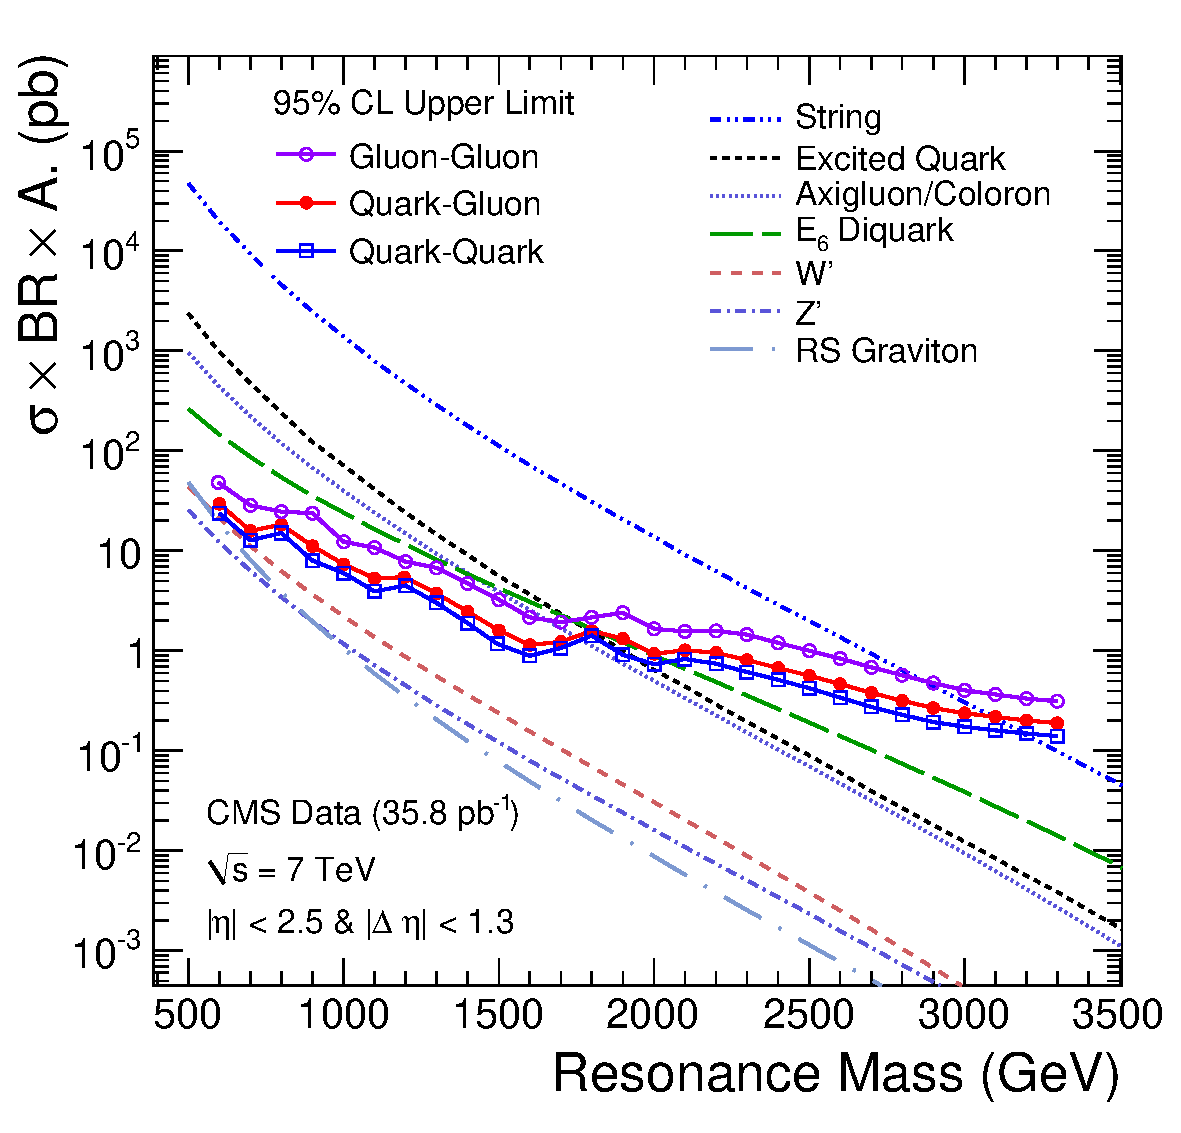
\includegraphics[width=\textwidth]{Figures/Limit_Comp_final.pdf}
    \caption{ The 95\% CL upper limits on the cross section for 
    dijet resonances (points) shown seperately for the three different 
    parton pairs $qq$, $qg$ and $gg$, is 
    compared to the model cross section for 7 different models (see text).}
    \label{limit_sys}
  \end{center}
\end{figure}


\begin{table}[htbH]
\centering
\large
\begin{tabular}{|c|c|c|c|}\hline
Mass   &  \multicolumn{3}{c|}{95\% C.L. $\sigma\cdot B$ (pb)}\\
 ($TeV$) &  quark-quark      & quark-gluon  & gluon-gluon\\ \hline
0.5	 &  118	         &  134	         &  206  \\  
0.6	 &  182	         &  229	         &  339  \\  
0.7	 &  90.7         &  134	         &  281  \\  
0.8	 &  70.8	 &  93.5	 &  177  \\  
0.9	 &  52.7	 &  71.6	 &  142  \\  
1.0	 &  20.3	 &  29.0	 &  71.4 \\  
1.1	 &  17.0	 &  20.1	 &  35.1 \\  
1.2	 &  17.0	 &  20.4	 &  32.5 \\  
1.3	 &  10.5	 &  12.9	 &  22.8 \\  
1.4	 &  6.77	 &  8.71	 &  16.4 \\  
1.5	 &  3.71	 &  5.02	 &  10.3 \\  
1.6	 &  3.05	 &  3.72	 &  6.71 \\  
1.7	 &  3.13	 &  3.64	 &  5.88 \\  
1.8	 &  2.92	 &  3.41	 &  5.37 \\  
1.9	 &  2.73	 &  3.15	 &  4.78 \\  
2.0	 &  2.71	 &  3.02	 &  4.39 \\  
2.1	 &  2.50	 &  2.84	 &  4.15 \\  
2.2	 &  2.20	 &  2.55	 &  3.69 \\  
2.3	 &  1.96	 &  2.28	 &  3.32 \\  
2.4	 &  1.79	 &  2.08	 &  2.94 \\  
2.5	 &  1.67	 &  1.93	 &  2.74 \\
2.6      &  1.55         &  1.80         &  2.50  \\
\hline
\end{tabular}
\caption{As a function of resonance mass we list our 95\% C.L. upper limit on
cross section times branching ratio for narrow resonances originating from   
quark-quark, quark-gluon, and gluon-gluon pairs of partons,
including systematic uncertainties.}
\label{tabXsecLimit}
\end{table}


\begin{figure}[!ht]
  \begin{center}
    \includegraphics[width=\textwidth]{Figures/model_over_limit}
    \caption{ The model cross section divided by the 95\% CL upper limits on the 
    cross section for the appropritate parton pairs.}
    \label{limit_ratio}
  \end{center}
\end{figure}



\clearpage
